\setlength{\parskip}{1pt} %% ESPAÇO DEPOIS DE 6pt
\pagenumbering{arabic}  %% PAGINAÇÃO INICIA AQUI
\setcounter{page}{16} % Reiniciar contagem de página para 1
%\pagestyle{plain} % Restaurar numeração de página com estilo "plain"
\clearpage
\pagestyle{fancy}


\section{Introdu{\c c}{\~a}o} \label{sec:int}

Este capítulo apresenta a introdução do que é abordado nesta dissertação, usando modelos ML, dentro destes modelos será abordada a previsão futura dos dados coletados na SANEPAR Curitiba no estado do Paraná, estes dados foram coletados no bairro superior nos anos 2018 a 2020 houve uma escassez de água que afetou a todos em Curitiba.

No uso de séries temporais pensando neste contexto de tomada de decisão, pode-se pensar como a aplicação de modelos ML em séries temporais, usando os modelos mais clássicos encontrados durante uma revisão não sistemática do conteúdo, para tabular alguns modelos que são usados na literatura.  




    \subsection{Contexto da pesquisa} \label{subsec:contexto}
\citeonline{mateus} A necessidade de desenvolvimento do planejamento estratégico no mundo corporativo e no dia-a-dia torna a análise de séries temporais e previsões valiosas ferramentas para apoiar o processo de tomada de decisão a curto, médio e longo prazo. Devido a não linearidades, sazonalidade, tendência e ciclicidade nos dados temporais, o desenvolvimento de modelos de previsão eficientes é uma tarefa desafiadora. 

 Em séries temporais, o aprendizado de máquina é frequentemente utilizado para processamento de big data, com o conjunto de dados da SANEPAR em Curitiba - PR, na cidade há algum consumo e escassez de água, é necessário avaliar os dados para ter certeza do que está acontecendo, quando há escassez d'água, e picos que ocorrem entre horas e dias.
 
 Dentre os modelos preditivos que serão apresentados em uma revisão sistemática, avaliar o melhor modelo que podemos utilizar e validar quando e como ocorre a escassez d'água. Estas análises será em \textit{python}.
 
 Explorar o que são séries temporais e aprendizado de máquina, séries temporais são dados armazenados ao longo do tempo que permitem ao observador analisar anomalias nos dados. Em séries temporais, ordenar os dados por ano ou dia é fundamental e, se os dados atribuídos de forma aleatória, assim podendo tornar mais difícil prever e tomar decisão baseado nos dados coletados. 
 Analisar médias pode ser bem perigoso se não excluir pontos fora da curva também conhecidos como \textit{outliers}. Pode gerar dados muito positivos ou negativos que não correspondem a realidade.
   
      
\subsubsection{Motiva\c c\~ao da pesquisa} \label{subsubsec:motivacao}
   %Escrever algo motivador 
    
    De acordo com \cite{vasconcelos_2020} Curitiba e região metropolitana enfrentou um rodízio com $36$ horas com água e $36$ horas sem abastecimento. A média geral dos reservatórios da região está em $27,96\%$ da capacidade. Assim em medida a isso essa pesquisa tem como a abordagem da falta de água, essa falta que pode ser vista como uma seca, em média nos anos anteriores de 2020 a chuva tem marcado a quantia de $1.704$ mm. \cite{vasconcelos_2020} Desde 2016, quando registrou 1.704 mm de chuva, Curitiba não atingiu mais a média anual de precipitação, que é de 1.490 mm, com base em dados da estação pluviométrica do Instituto Nacional de Meteorologia (Inmet).  Apesar de abaixo da média, o mínimo registrado desde então ocorreu em 2020, com 1.158 mm.
    
    Em mediano a essa motivação pode ser melhor interpretado os dados que a SANPEAR ofertor para prever e evitar a escasseia de água que foi registada, e a anomalia que foi detectado em 2020, com a volta da chuva os reservatórios teve aumento do nível.
    
          
    \subsection{Objetivo Geral} \label{subsec:objetivos}

O objetivo desta pesquisa é identificar o modelo de aprendizado de máquina mais adequado para previsão de séries temporais. 

Ao longo da dissertação, serão avaliados diversos modelos de regressão, com destaque para os modelos de redes neurais e o Prophet. É importante mencionar que a pesquisa enfatizará os modelos de \textit{gradient boosting}, além do ARIMA e suas variações mais contemporâneas. Além das previsões, também serão realizadas análises de anomalias nos dados, buscando compreender as causas subjacentes a essas ocorrências.
 
    
    
    \subsubsection{Objetivos Espec\'ificos e Quest\~ao de Pesquisa} \label{subsubsec:obespec}
    
Neste estudo, busca-se identificar e compreender possíveis anomalias nos dados, bem como investigar as causas por trás dessas ocorrências. Entre os objetivos específicos está responder às perguntas de pesquisa relacionadas a essas anomalias.

\begin{enumerate}[start=1, label={\textbf{Q} \arabic*}]
	\item \label{q1} Qual é a adequação da pressão atual para atender à demanda diária?
	\item \label{q2} Qual é o volume mínimo de água necessário no reservatório para evitar o acionamento das bombas durante o horário de pico? 
	\item \label{q3} Qual é a vazão ótima para atender à demanda diária?
	\item \label{q4} Como encontrar o ponto de equilíbrio entre a demanda e a vazão?
	\item \label{q5} Qual é o impacto do acionamento das bombas durante o horário de pico?
	 
	\begin{enumerate}[label=\alph*.]
	\item \label{q5:a} Qual é o nível ideal no reservatório para evitar a ativação das bombas da SANEPAR durante o período de maior demanda, das 18h às 21h, sem comprometer o abastecimento de água para a população?  
	\item \label{q5:b} Existe tendência, padrão, sazonalidade para os dados destes três anos do Bairro Alto?
	\item \label{q5:c} Identificar quais os horários de maior demanda das $18$ às $21$?
	\item \label{q5:d} Quanto deve-se armazenar previamente no reservatório para não acionar as bombas no horário de pico?
	\item \label{q5:e} Se a vazão cresce e a pressão decresce existe uma ANOMALIA na rede (com base no histórico).	
	\end{enumerate}
\end{enumerate}

    
    \subsection{Descri\c c\~ao do problema} \label{subsec:descricao}

A descrição do problema é fundamental para obter uma compreensão mais precisa do que está sendo abordado neste trabalho. É por meio dessa descrição que as variáveis-chave são expostas e o objetivo da previsão é estabelecido de forma clara. Sem um plano estruturado para determinar o que deve ser previsto, torna-se difícil justificar o uso de modelos de previsão de dados. Portanto, é essencial estabelecer um propósito claro e definir as metas da previsão antes de aplicar os modelos adequados.

\begin{itemize}
	\item Bombas de sucção (B1, B2 e B3) – valor máximo da frequência 60 Hz
	
	\item[] Variáveis importantes: Fluxo, pressão e nível
	
	\item Nível do Reservatório (Câmara 1) LT01 $ (m^3) $ - \textbf{PREVER}
	
	\item Vazão de entrada (FT01) $ (m^3/h) $
	
	\item Vazão de gravidade (FT02) $ (m^3/h) $
	
	\item Vazão de recalque (FT03) $ (m^3/h) $
	
	\item Pressão de Sucção (PT01SU) (mca)
	
	\item Pressão de Recalque (PT02RBAL) (mca)
\end{itemize}

A pesquisa fará uso da variável LT01, que representa o nível do reservatório e desempenha um papel de extrema importância, como evidenciado pelas Figuras \ref{fig:dados-todos} e \ref{fig:2020-a-frente}. Essas figuras retratam as anomalias ocorridas durante o período em que a capital paranaense foi afetada pela escassez de chuvas, resultando na redução do nível dos reservatórios e na implementação de rodízios periódicos, conforme discutido na subseção \ref{subsubsec:motivacao}. Assim, tais observações permitem uma compreensão mais aprofundada das perspectivas futuras.

\subsection{Procedimentos metodol{\'o}gicos} \label{subsec:metod}

Com o intuito de realizar previsões e fazer comparações entre os modelos obtidos na revisão sistemática, será adotado um processo metodológico bem definido. Tal processo está detalhado na subseção \ref{subsubsec:etp} desta seção, onde foram estabelecidas as etapas a serem seguidas desde o início. Isso inclui a definição do que será previsto, bem como a seleção dos métodos a serem utilizados na Análise Exploratória de Dados (EDA), seguindo uma sequência lógica e coerente.
   
    \subsubsection{Etapas da pesquisa}\label{subsubsec:etp}

    
    A pesquisa seguiu as seguintes etapas:
    \begin{figure}[H]
    	\centering
    	\caption{Mapa das Etapas}
    	\label{fig:etapas}
    	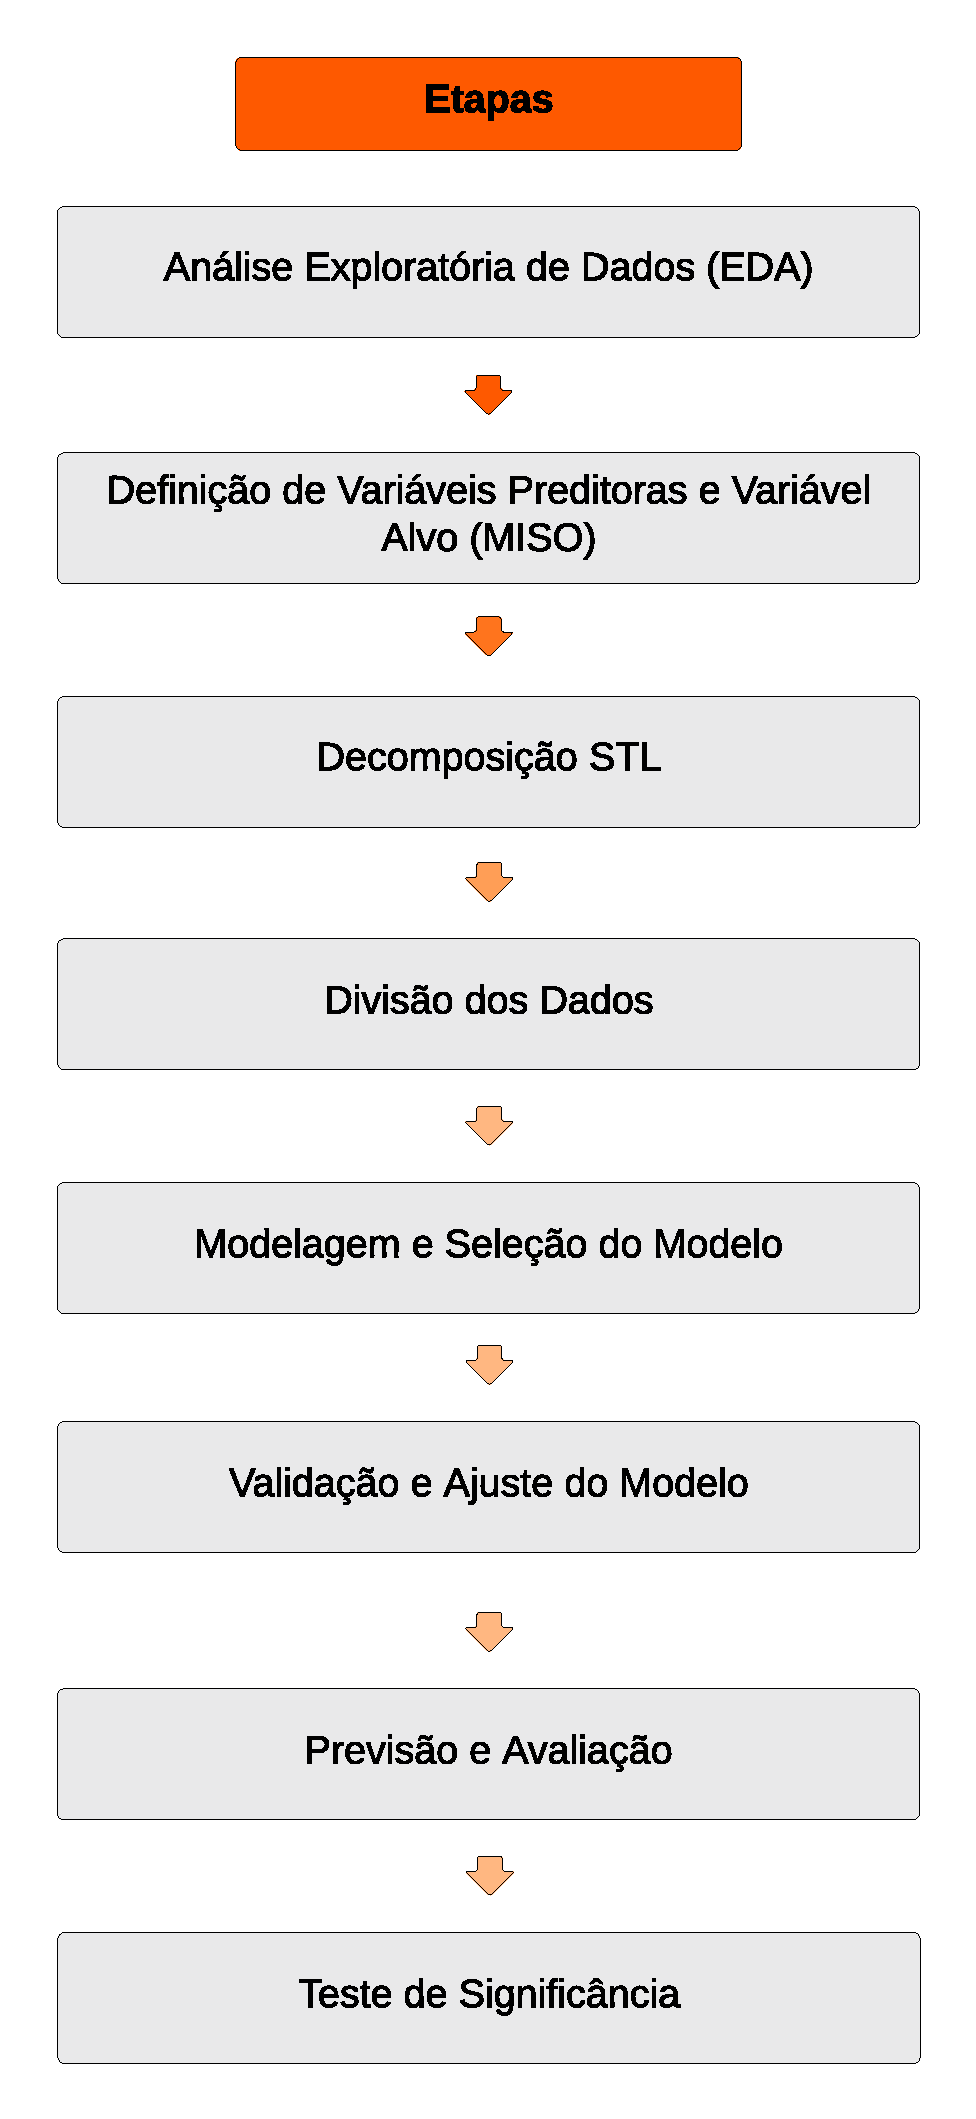
\includegraphics[width=1\linewidth]{Introducao/Figuras/Etapas}
    	
    	\fonte{Elaboração própria}
    \end{figure}
    \begin{enumerate}[start=1, label = {\textbf{Etapa} \arabic*} ]
    	\item Análise exploratória dos dados – EDA ( do inglês \textit{Exploratory Data Analysis}). \label{etp:1}
    	
    	A exploração de dados na EDA é fundamental para entender melhor os dados que estão sendo trabalhados, como, por exemplo, excluir valores ausentes, saber como os dados estão separados em horas ou dias e, assim, tomar a melhor decisão a ser trabalhada com os dados, usar gráficos de linha na análise para observar a convergência dos dados e as anomalias que podem ocorrer.
    	
        	
    	\item O que vai ser usado como variáveis previsoras e qual será a variável a ser predita (MISO). \label{etp:2}
    	
    	Nessa etapa, tem o papel de relacionar as variáveis ao que será previsto, como os modelos de variáveis exógenas que são usados aqui nos modelos SARIMAX, ARX e ARIMAX do tipo ARIMA. Cada modelo tem a interação de mais variáveis do que o modelo ARIMA básico ou seus derivados AR, MA e SARIMA. O conhecimento de quais variáveis estão incluídas na modelagem do problema torna a modelagem mais abrangente quando o horizonte de previsão é estendido além dos dados.
    	
       	
    	\item Fazer a decomposição STL (do inglês \textit{Seasonal-Trend Decomposition}) Sazonalidade, Tendência e Resíduo. \label{etp:3}
    	
    	\citeonline{en15165875} destacam que ``o uso do método de decomposição STL em conjunto com um modelo híbrido se mostrou eficaz na previsão de carga de curto prazo'' (p. 6).
    	
    	Segundo \citeonline{inproceedings}, ``a aplicação da decomposição STL e do modelo LSTM baseado em atenção foi capaz de prever com precisão a velocidade do tráfego de curto prazo'' (p. 6).
    	
    	\citeonline{su13041694} afirmam que ``a combinação da decomposição STL e modelos de aprendizado profundo mostrou-se promissora na previsão de carga de eletricidade'' (p. 18).
    	
        O algoritmo STL executa suavização na série de tempo usando LOESS em dois loops; o loop interno itera entre a suavização sazonal e de tendência e o loop externo minimiza o efeito de valores atípicos. Durante o loop interno, o componente sazonal é calculado primeiro e removido para calcular o componente de tendência. O restante é calculado subtraindo os componentes sazonais e de tendência da série de tempo.
        
        Os três componentes da análise STL se relacionam com a série de tempo bruta da seguinte forma:
        
        \begin{align}
        	y_i &= s_i + t_i + r_i\label{eq:stl1}
        \end{align}
    	
    	Da equação \eqref{eq:stl1}:
    	
    	\begin{itemize}
    		\item $y_i = O$ valor da série de tempo no ponto $i$.
    		\item $s_i = O$ valor do componente sazonal no ponto $i$.
    		\item $t_i = O$ valor do componente de tendência no ponto $i$.
    		\item $ri = O$ valor do componente restante no ponto $i$.
    	\end{itemize}
    	\item \label{etp:4} Separação dos dados.
    	
  
    De acordo com a literatura acadêmica, é comum dividir o conjunto de dados em treinamento, validação e teste para avaliar a performance dos modelos. Essa abordagem permite uma análise mais completa do desempenho do modelo, garantindo uma avaliação objetiva de sua capacidade de generalização e evitando problemas de overfitting ou subajuste \cite{cruz-ramirez2020enhancing,mokhtari2020deep,khan2021hybrid,sharma2021deep}.
    
    A fim de obter uma divisão mais adequada dos dados, é realizado um estudo das medidas de tendência central e dispersão de cada conjunto. O conjunto de dados é então dividido em três partes distintas: treinamento, validação e teste. Nessa divisão, inicialmente, 70\% dos dados são utilizados para o treinamento e validação, enquanto os 30\% restantes são reservados para o conjunto de teste. Em seguida, a porção destinada ao treinamento e validação é subdividida em uma proporção de 80\% para treinamento e 20\% para validação.
    	
    	
    	\item Estratégia de previsão (recursiva e iterada-método direto). \label{etp:5}
    	
    	A estratégia recursiva é mencionada por \citeonline{PETROPOULOS2022705} como uma abordagem eficaz na previsão de séries temporais de múltiplos passos. De acordo com o autor, essa estratégia envolve o uso de previsões anteriores como entradas para prever os próximos passos da série temporal. A abordagem recursiva tem demonstrado potencial para melhorar a acurácia das previsões de séries temporais de longo prazo.
    	
    	A estratégia recursiva consiste em utilizar um modelo de previsão de um passo de tempo várias vezes, onde a previsão obtida no passo anterior é utilizada como entrada para realizar a previsão do próximo passo de tempo.
    	
    	No contexto da previsão da demanda de água para os próximos dias, seria desenvolvido um modelo de previsão de um único passo. Esse modelo seria aplicado para prever a demanda no primeiro dia e, em seguida, essa previsão seria utilizada como dado de entrada para prever a demanda do segundo dia. Esse processo se repetiria para os demais dias, permitindo a previsão da demanda ao longo do tempo.
    	    		 
    	Por Exemplo:
    	
    	\begin{eqnarray}
    	preditivo(t+1) &=& model_1(obs(t-1), obs(t-2), \ldots, obs(t-n))\\
    	preditivo(t+2) &=& model_2(obs(t-2), obs(t-3), \ldots, obs(t-n))   	
    	\end{eqnarray}
    	
    	\citeonline{machinemaster} como as previsões são usadas no lugar das observações, a estratégia recursiva permite que os erros de previsão se acumulem de tal forma que o desempenho possa se degradar rapidamente à medida que o horizonte de tempo de previsão aumenta.
    	
    	
    	\item Horizonte de previsão (1 passo ou n passos à frente). \label{etp:6}
    	
    	Para abordar a diversidade de horizontes de previsão, optou-se por considerar diferentes intervalos de tempo. Isso permitirá a realização de previsões para um passo à frente, uma semana, duas semanas e um mês, de forma a abranger distintas perspectivas de curto e médio prazo. Essa abordagem proporciona uma análise abrangente da capacidade dos modelos em lidar com horizontes de previsão variados, contribuindo para uma avaliação mais completa e precisa do desempenho dos mesmos.
    	
    	
    	\item Modelos de previsão e métricas de desempenho. \label{etp:7}
    	
    	Os modelos abordados nesta pesquisa são tanto os modelos clássicos de previsão quanto os modelos de regressão por gradiente. Entre os modelos clássicos, incluem-se o AR, ARX, ARMA, ARIMA, SARIMA, SARIMAX e ARIMAX, enquanto os modelos de regressão por gradiente englobam o LR, XGBRegressor, RFR e LGBMRegressor. A seleção desses modelos foi baseada em uma revisão sistemática realizada durante a dissertação, buscando identificar os modelos mais eficazes e amplamente utilizados na literatura.
    	
    	Ao longo da pesquisa, foram adotadas três métricas principais para avaliar o desempenho dos modelos: RRMSE, MAE  e sMAPE. Essas métricas foram escolhidas com base na revisão sistemática e são amplamente reconhecidas como medidas de qualidade de previsão. Cada métrica tem sua própria interpretação e importância, sendo detalhada na subseção \ref{subsec:metrica} para um melhor entendimento de como são aplicadas e interpretadas na pesquisa.
    	
    	
    	
    	%\item Ajustar os hiperparâmetros dos modelos de previsão Hiperparâmetro ajusta a priori (ex: número de neurônios da rede neural), e parâmetro (pesos da rede neural) ajusta durante o processo. \label{etp:8}
    	
    	
    	\item Aplicar os modelos de previsão e fazer comparativo baseado em testes de significância estatística (\textit{Friedman e Nemenyi}). \label{etp:9}
    	
    	
    	O teste de Friedman é o teste não paramétrico usado para comparar dados de amostras vinculadas, ou seja, quando o mesmo indivíduo é avaliado mais de uma vez. 
    	ou seja, quando o mesmo indivíduo é avaliado mais de uma vez. 
    	O teste de Friedman não usa os dados numéricos diretamente, mas sim as classificações ocupadas pelos dados após a classificação de cada grupo separadamente. 
    	separadamente. Após a classificação, a hipótese de igualdade da soma das classificações de cada grupo é testada. 

		O teste consiste em fazer comparações em pares com o intuito de verificar qual dos fatores que diferem entre si. No entanto, o teste de Nemenyi é muito conservador e pode não encontrar diferença significativa entre os pares testados.
    	
    \end{enumerate}






    
    
    \subsection{Justificativa da Pesquisa} \label{subsec:justif}

Ao longo desta dissertação, os seguintes aspectos são abordados visando a previsão e tomada de decisões.

\subsubsection{Contribui\c c\~oes} \label{subsubsec:Contribuição}

As perguntas de pesquisa apresentadas na subseção \ref{subsubsec:obespec}, surgem duas contribuições significativas nesta dissertação. A primeira diz respeito à previsão da demanda de água na cidade de Curitiba, abordando aspectos como consumo e gasto de energia durante períodos de pico.

Segundo estudos recentes, os modelos ARIMA desempenham um papel fundamental na análise de séries temporais. Os modelos ARIMA são utilizados na previsão de séries temporais devido à sua capacidade de capturar padrões complexos e comportamentos de longo prazo \cite{arima_python}.

Conforme relatos, o modelo XGBoost tem sido aplicado com sucesso em problemas de previsão de séries temporais. Estudos demonstraram que o XGBoost é uma ferramenta para lidar com desafios de previsão em séries temporais \cite{xgboost_intro}. O LightGBM tem ganhado destaque como um modelo eficiente para previsão de séries temporais \cite{WELLENS20221482}. De acordo com \citeonline{decisiontree}, o algoritmo de árvore de decisão é um dos mais populares e eficazes na área de classificação. Alguns modelos baseados em árvores possuem eficiência computacional e são capazes de lidar tanto com dados categóricos quanto numéricos. Já \citeonline{random_forest_regression} enfatiza a importância do uso de \textit{Random Forest Regression} na previsão de séries temporais.

As RNNs (Redes Neurais Recorrentes) são redes neurais artificiais que possibilitam o processamento de dados sequenciais. Elas são amplamente utilizadas em mineração de dados e aprendizado de máquina devido à sua habilidade em modelar dependências temporais \cite{rnn}. Assim como outras redes neurais artificiais, as RNNs são capazes de lidar com a detecção de anomalias de forma mais eficaz do que modelos mais básicos de séries temporais, como o modelo ARIMA e seus predecessores. Enquanto o ARIMA pode identificar anomalias nos dados, as RNNs podem ajustar e otimizar os neurônios para aumentar a eficácia na detecção dessas anomalias.

As CNNs (Redes Neurais Convolucionais) representam uma classe de redes neurais profundas amplamente utilizadas em tarefas de reconhecimento de imagens e vídeos \cite{cnn}. Embora sejam uma opção vantajosa para previsões de tempo, assim como as RNNs, as CNNs são especialistas em dados bidimensionais. Isso pode resultar em erros maiores quando comparadas às RNNs em contextos de dados sequenciais.

As GRUs (Unidades Recorrentes com Portões)  são um tipo de rede neural recorrente introduzido como alternativa às LSTMs (Unidades de Memória de Longo e Curto Prazo) \cite{gru}. As LSTMs, por sua vez, foram desenvolvidas para resolver o problema do gradiente desvanecido em RNNs padrão \cite{lstm}. Embora sejam semelhantes às RNNs, as GRUs e LSTMs incorporam técnicas específicas para melhorar a capacidade das RNNs em lidar com dependências temporais a longo prazo. Cada uma delas possui particularidades que as tornam mais adequadas para diferentes cenários de previsão, com a GRU sendo especialmente útil para resolver problemas relacionados à dissipação de gradientes.


Constata-se que as redes GRU demonstram uma vantagem em relação às redes LSTM em termos de complexidade e desempenho. As RNN, incluindo tanto GRU quanto LSTM, são observadas como tendo uma capacidade competitiva em tarefas de aprendizagem de sequências. Portanto, os resultados sugerem que as redes GRU, pertencentes à categoria de RNN, são mais adequadas para a aprendizagem de sequências simbólicas que exigem memória seletiva e adaptativa \cite{DBLP:journals/corr/abs-2107-02248}.

No entanto, de acordo com as constatações dessa pesquisa, o modelo RNN especificamente o GRU é identificado como o melhor modelo para a tarefa em questão. Isso se baseia na habilidade do GRU em eficientemente memorizar e generalizar sequências, resultando em um desempenho superior em comparação a outros modelos, incluindo ANN (do inglês \textit{Artificial Neural Network}), CNN e modelos baseados em gradientes, tais como XGBoost e LightGBM. Dessa forma, conclui-se que o modelo RNN, e mais especificamente o GRU, se destaca como a escolha mais apropriada para a aprendizagem e previsão de séries temporais.



    
    \subsection{Estrutura do trabalho} \label{subsec:estrutura}

 Este documento está estruturado em~\ref{sec:conclusoes} capítulos, divididos da seguinte forma:
   
    \begin{figure}[H]
    	\centering
    	\caption{Estrutura da dissertação}
    	\label{fig:estrutura}
    	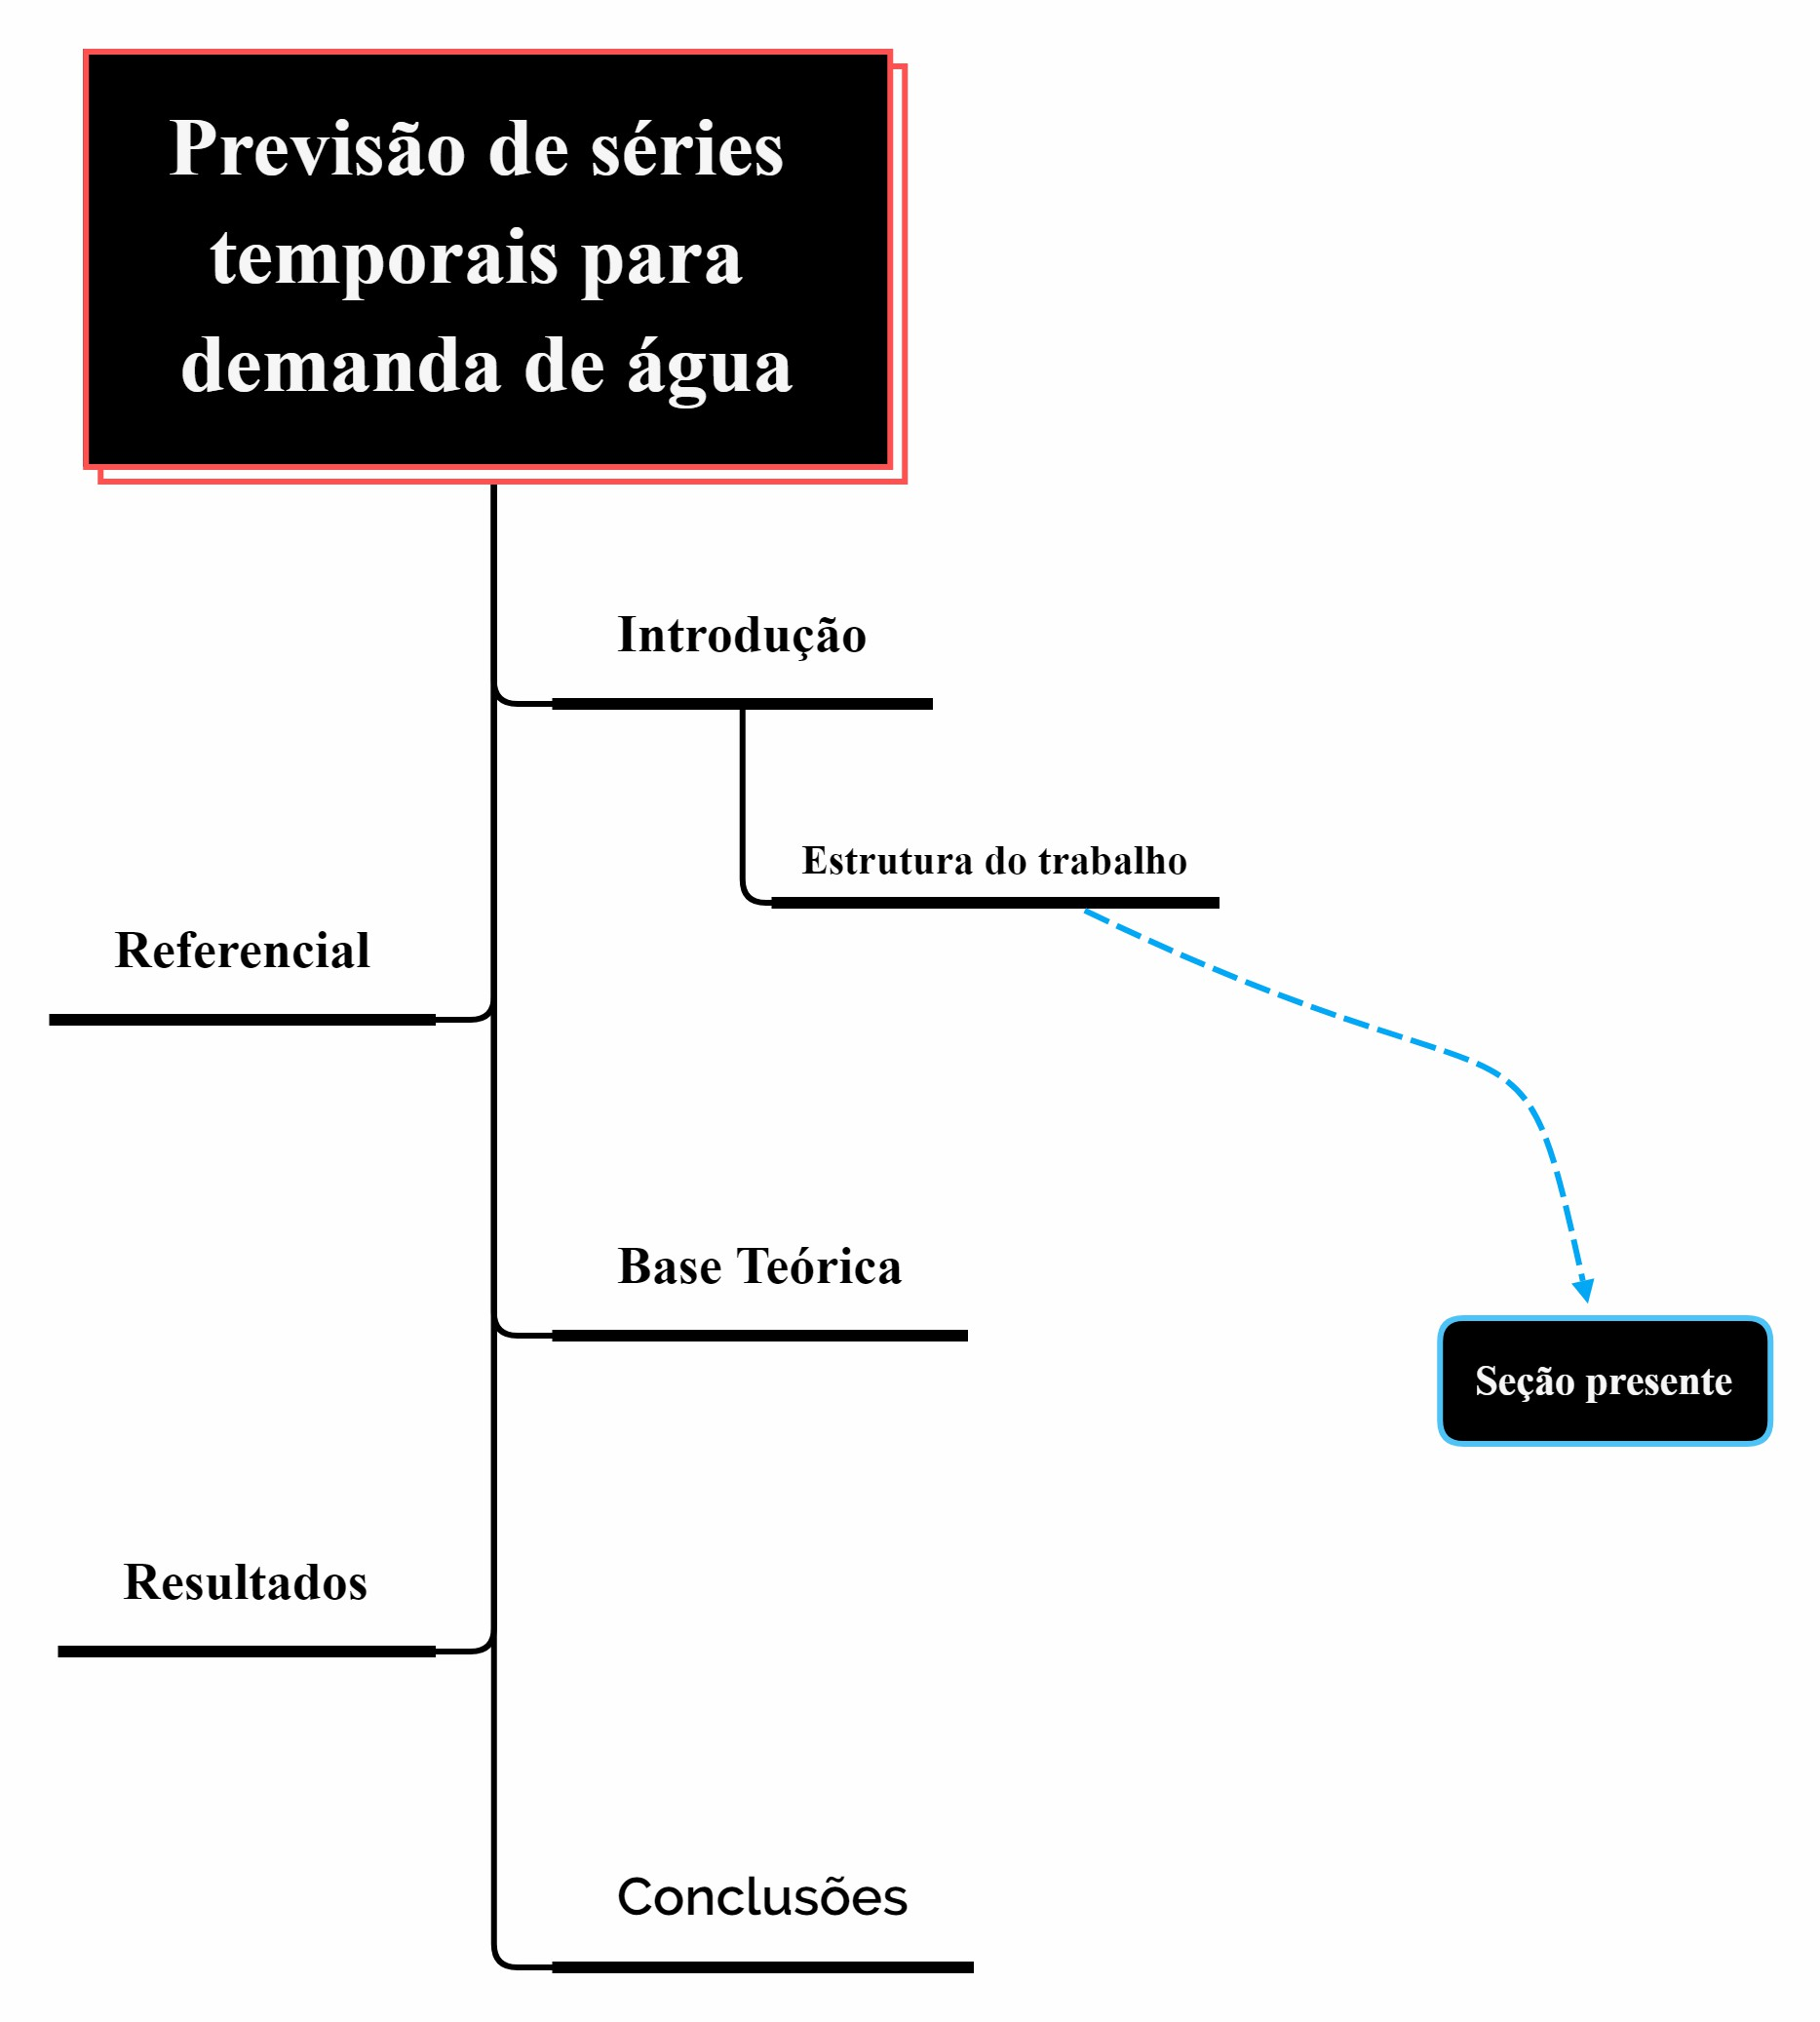
\includegraphics[width=0.7\linewidth]{Introducao/Figuras/Estrutura}
    	
    	Fonte: Elaboração própria 
    \end{figure}
O capítulo~\ref{sec:int} apresenta a introdução do trabalho, contendo a contextualização, a motivação, o objetivo geral, os objetivos específicos e a questão de pesquisa, a descrição do problema, a metodologia utilizada, a justificativa da pesquisa, as contribuições e a organização do trabalho.
O capítulo~\ref{sec:refteo} revisão teórica do trabalho, fazendo uma visão geral dos principais pesquisadores sobre as questões abordadas na pesquisa.
O capítulo~\ref{sec:base} apresenta os modelos que serão trabalhados nos dados coletados.
O capítulo~\ref{sec:result} apresenta os resultados da pesquisa, assim como uma análise dos resultados gerados.
O capítulo~\ref{sec:conclusoes}, finalmente, apresenta as considerações finais da pesquisa e algumas propostas para pesquisas futuras.



    